\documentclass{standalone}
\usepackage{tikz}
\usetikzlibrary{automata,positioning}

\begin{document}
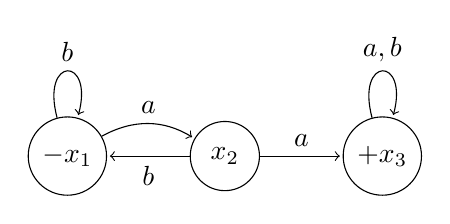
\begin{tikzpicture}[shorten >=1pt,node distance=2cm,on grid,auto]
  \node[state] (q_1) {$-x_1$}; 
  \node[state] (q_2) [right of=q_1] {$x_2$}; 
  \node[state] (q_3) [right of=q_2] {$+x_3$}; 

  \path[->] 
    (q_1) edge [loop above] node {$b$} (q_1)
    (q_1) edge [bend left] node {$a$} (q_2)
    (q_2) edge node {$a$} (q_3)
    (q_2) edge node {$b$} (q_1)
    (q_3) edge [loop above] node {$a,b$} (q_3);
\end{tikzpicture}
\end{document}